\documentclass[a4paper, 12pt]{article}

% Margins
\topmargin=-0.45in
\evensidemargin=0in
\oddsidemargin=0in
\textwidth=6.5in
\textheight=9.0in
\headsep=0.25in 

%package usage
\PassOptionsToPackage{svgnames}{xcolor}
\usepackage[colorlinks=true, citecolor=blue, linkcolor=purple]{hyperref}
\usepackage[english]{babel}
\usepackage[latin1]{inputenc}
\usepackage{enumitem}
\usepackage{indentfirst}
\usepackage{colortbl}
\usepackage{longtable}
\usepackage{animate}
\usepackage{threeparttablex}
\usepackage{etoolbox}
\usepackage{rotating}
\usepackage{multirow}
\usepackage{pdflscape}
\usepackage{tablefootnote}
\usepackage[table,xcdraw]{xcolor}
\usepackage{amsmath}
\usepackage{flafter} 
\usepackage{dcolumn} 
\usepackage{natbib}
\usepackage{rotating}	
\usepackage{adjustbox}
\usepackage{amsthm}
\usepackage{graphicx}
\usepackage{amssymb}
\usepackage{tcolorbox}
\usepackage{lipsum}
\usepackage{tikz}
\usepackage{tabularx}
\tcbuselibrary{skins,breakable}
\usetikzlibrary{shadings,shadows}
\usepackage{threeparttable}
\usepackage{subfig}
\usepackage{setspace}
\usepackage{booktabs}
\usepackage{placeins}
\usepackage{enumitem}
\usepackage{natbib}
\usepackage{filecontents}
\usepackage[encoding,filenameencoding=utf8,extendedchars,space]{grffile}
\newcommand{\addfig}[2]{\begin{center}
			\includegraphics[width=#1\textwidth]{#2}
	\end{center}
}

%\usepackage[capposition=top]{floatrow}
%\usepackage[colorinlistoftodos]{todonotes}
\newcommand{\expect}[2]{\mathbb{E}_{#2}\left(#1\right)}

\newtheorem{theorem}{Theorem}[section]
\newtheorem{corollary}{Corollary}[theorem]
\newtheorem{proposition}[theorem]{Proposition}

\newcommand{\alert}[1]{{\textbf{\color{red}#1}}}
%general commands

\newcommand{\bcite}{\begin{quote}}
\newcommand{\ecite}{\end{quote}}
\newcommand{\beqns}{\begin{eqnarray*}}
\newcommand{\eeqns}{\end{eqnarray*}}
\newcommand{\beqn}{\begin{eqnarray}}
\newcommand{\eeqn}{\end{eqnarray}}
\newcommand{\benu}{\begin{enumerate}}
\newcommand{\eenu}{\end{enumerate}}
\newcommand{\bitem}{\begin{itemize}}
\newcommand{\eitem}{\end{itemize}}
\newcommand{\smallGap}{\vspace{.25cm}}

\newenvironment{block}[1]{%
	\tcolorbox[beamer,%
	noparskip,breakable,
	colback=LightGreen,colframe=DarkGreen,%
	colbacklower=LimeGreen!75!LightGreen,%
	title=#1]}%
{\endtcolorbox}


\newcommand{\sym}[1]{\rlap{#1}}% Thanks David Carlisle

\usepackage{siunitx}
\sisetup{
	detect-mode,
	group-digits		= false,
	input-symbols		= ( ) [ ] - +,
	table-align-text-post	= false,
	input-signs             = ,
}

%mathematical commands
\newcommand{\problemIndustries}{(A_t\cup \Omega_t)}
\newcommand{\red}[1]{{\color{red}#1}}
\newcommand{\normalIndustries}{\problemIndustries^C}
\newcommand{\sumNormalIndustries}{\sum_{j\in\normalIndustries}}
\newcommand{\sumProblemIndustries}{\sum_{j\in\problemIndustries}}
\newcommand{\sumWithinNormal}{\sum_{j\in\normalIndustries\cap \Gamma_t}}
\newcommand{\sumWithinProblem}{\sum_{j\in\normalIndustries\cap \Gamma_t^C}}
\newcommand{\ser}[1]{s_{er#1}}
\newcommand{\cov}{\text{cov}}
\newcommand{\explain}[2]{\underbrace{#1}_{\parbox{\widthof{\ensuremath{#1}}}{\footnotesize\raggedright #2}}}
\newcommand{\lfpthresh}[1]{\underline{\chi_{#1 lt}}}
\newcommand{\crho}{\frac{\sigma-1}{\sigma}}
\newcommand{\crhoinv}{\frac{\sigma}{\sigma-1}}

\newcommand{\lquote}[3][]{\bcite #2 \citep[#1]{#3} \ecite}

\newcommand{\laquote}[3][]{\bcite #2 \citepalias[#1]{#3} \ecite}
\usepackage{tabularx}

\begin{document}
	\section{Education}
%	\bitem
%	\item I group education levels by looking at how similar the occupational distribution between them.
%	\item I do this by examining:
%		\bitem
%		\item Correlation of the employment distribution across skills.
%		\item Computing the pairwise Welch indexes:
%	
%		\eitem
	\bitem
	\item I do the grouping as follows:
	\bitem 
	\item Low education: no qualification,  GCSE D-G, and  GCSE A-C.
	\item Medium education:  GCSE A*.
	\item High education: Bachelor +.
	\eitem
	
	\item The Welch index is computed as:
		\begin{align*}
		G_{kl}&=\frac{\sum_o(q_{ko}-\bar{q}_{o})(q_{lo}-\bar{q}_{c})/\bar{q_o}}{\sqrt{(\sum_o(q_{ko}-\bar{q}_o)^2/\bar{q}_o)(\sum_o(q_{lo}-\bar{q}_o)^2/\bar{q}_o)}}
		\end{align*}
	where $k,l$ denote education levels, $o$ occupation, $q_{ko}$ denotes the share of k-people employed in occupation $o$, and $\bar{q}_o$ is the share of population employed in job $o$.
	\eitem
	
	% Table generated by Excel2LaTeX from sheet 'correlationLFS'
\begin{table}[htbp]
	\centering
	\caption{Welch index of the occupational distribution of employment}
	\begin{tabular}{c|rrrrr}
		& \multicolumn{1}{c}{\textbf{None}} & \multicolumn{1}{c}{\textbf{GCSE D-G}} & \multicolumn{1}{c}{\textbf{GCSE A-C}} & \multicolumn{1}{c}{\textbf{GCE A*}} & \multicolumn{1}{c}{\textbf{Bachelor's +}} \\
		\midrule
		\textbf{None} & 1.000 &       &       &       &  \\
		\textbf{GCSE D-G} & \cellcolor[rgb]{ .973,  .412,  .42}0.736 & 1.000 &       &       &  \\
		\textbf{GCSE A-C} & \cellcolor[rgb]{ .988,  .655,  .467}0.356 & \cellcolor[rgb]{ .984,  .588,  .455}0.462 & 1.000 &       &  \\
		\textbf{GCE A*} & \cellcolor[rgb]{ .965,  .91,  .514}-0.106 & \cellcolor[rgb]{ 1,  .898,  .514}-0.031 & \cellcolor[rgb]{ .992,  .745,  .486}0.215 & 1.000 &  \\
		\textbf{Bachelor's +} & \cellcolor[rgb]{ .482,  .769,  .486}-0.659 & \cellcolor[rgb]{ .424,  .753,  .482}-0.723 & \cellcolor[rgb]{ .388,  .745,  .482}-0.767 & \cellcolor[rgb]{ .627,  .812,  .494}-0.491 & 1.000 \\
	\end{tabular}%
	\caption*{\footnotesize\textit{Source:} UK LFS 1997-2017}
\end{table}%
	% Table generated by Excel2LaTeX from sheet 'correlationLFS'
\begin{table}[h!]
	\centering
	\caption{Correlation of occupational distribution of employment by education level}
	\begin{tabular}{c|ccccc}
		& \textbf{None} & \textbf{GCSE D-G} & \textbf{GCSE A-C} & \textbf{GCE A*} & \textbf{Bachelor's +} \\
		\midrule
		\textbf{None} & 1.000 &       &       &       &  \\
		\textbf{GCSE D-G} & \cellcolor[rgb]{ .973,  .412,  .42}0.862 & 1.000 &       &       &  \\
		\textbf{GCSE A-C} & \cellcolor[rgb]{ .988,  .69,  .475}0.689 & \cellcolor[rgb]{ .98,  .51,  .439}0.801 & 1.000 &       &  \\
		\textbf{GCE A*} & \cellcolor[rgb]{ .918,  .898,  .51}0.481 & \cellcolor[rgb]{ .996,  .827,  .502}0.600 & \cellcolor[rgb]{ .984,  .565,  .451}0.766 & 1.000 &  \\
		\textbf{Bachelor's +} & \cellcolor[rgb]{ .388,  .745,  .482}0.078 & \cellcolor[rgb]{ .506,  .776,  .486}0.168 & \cellcolor[rgb]{ .678,  .827,  .498}0.300 & \cellcolor[rgb]{ .725,  .839,  .498}0.334 & 1.000 \\
	\end{tabular}%
	\caption*{\footnotesize\textit{Source:} UK LFS 1997-2017}
\end{table}%

	\begin{center}
\begin{threeparttable}[!h]
\caption{Population by education level}
\label{tab:popcount}
\begin{tabular}{lccccc}
\toprule
\toprule
\textbf{Education level}&\multicolumn{1}{c}{\textbf{1997}}&\multicolumn{1}{c}{\textbf{2001}}&\multicolumn{1}{c}{\textbf{2006}}&\multicolumn{1}{c}{\textbf{2012}}&\multicolumn{1}{c}{\textbf{2017}} \\
\midrule
Low                 &        0.27&        0.27&        0.26&        0.25&        0.24&        0.24&        0.23&        0.22&        0.21&        0.20&        0.20&        0.20&        0.18&        0.17&        0.15&        0.14&        0.13&        0.13&        0.13&        0.13&        0.12\\
Medium              &        0.46&        0.46&        0.46&        0.46&        0.46&        0.46&        0.46&        0.46&        0.46&        0.45&        0.44&        0.45&        0.44&        0.43&        0.44&        0.44&        0.43&        0.43&        0.42&        0.41&        0.42\\
High                &        0.26&        0.28&        0.28&        0.29&        0.29&        0.30&        0.32&        0.32&        0.33&        0.35&        0.36&        0.36&        0.38&        0.40&        0.41&        0.43&        0.44&        0.44&        0.45&        0.46&        0.46\\
\midrule Total population (000)&      22,850&      23,163&      23,396&      23,706&      24,202&      24,507&      24,563&      24,835&      25,017&      25,186&      25,435&      25,354&      24,969&      25,082&      25,123&      25,474&      25,686&      26,297&      26,621&      26,834&      27,186\\
\bottomrule
\bottomrule
\end{tabular}
\begin{tablenotes}
\item \footnotesize \textit{Note:} uses data from UK LFS for the 4th quarter of each year. Table generated on 19 Jun 2020 at 11:59:20.
\end{tablenotes}
\end{threeparttable}
\end{center}


	\section{Boundary jobs}
	Let $s_{j}(o), j\in\{H,M,L\}$ denote the share $o$-workers with education level $j$. Denote as $p_i(o)$ the $i$-th largest element of $\{s_H(o),s_M(o),s_L(o)\}$.
	\bitem
	\item \textbf{Definition 1:} $o\in B_1$ iff (suggested by Costas):
	\beqns
	p_1(o)\leq R
	\eeqns
	\item \textbf{Definition 2:} $o\in B_2$ iff:
	\beqns
	\frac{p_1(o)}{p_1(o)+p_2(o)}\leq R
	\eeqns
	\item \textbf{Definition 3}: $o\in B_3$ iff (similar to 2, but generates border ``arms'' of constant width):
	\beqns
	p_1(o)-p_2(o)\leq R-0.5
	\eeqns
	\item For any $R$, $B_3\subset B_2\subset B_1$
	\eitem
	
	\begin{figure}[h!]
		\centering
		\caption{Border under alternative definitions}
		\subfloat[Definition 1:]{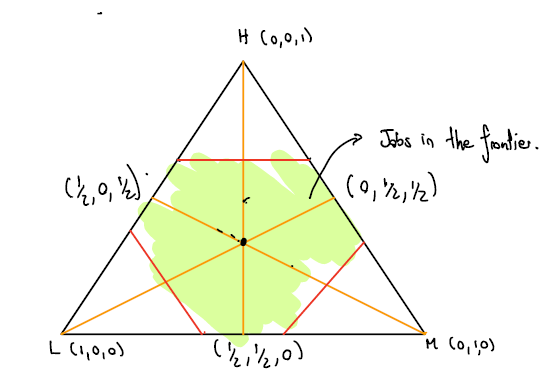
\includegraphics[width=.5\textwidth]{../output/absoluteFrontierDrawing}}
		\subfloat[Definition 2:]{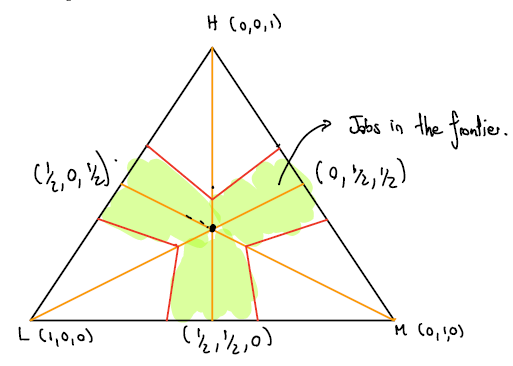
\includegraphics[width=.5\textwidth]{../output/relativeFrontierDrawing}}\\
		\subfloat[Definition 3:]{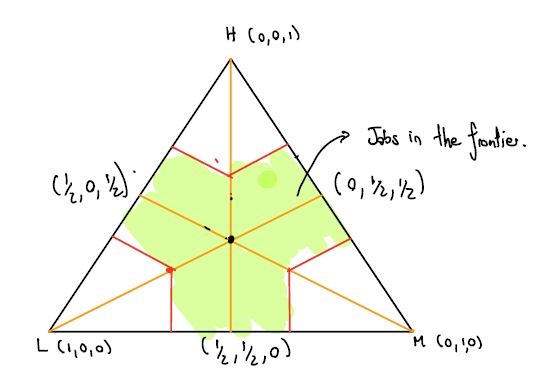
\includegraphics[width=.5\textwidth]{../output/parallelFrontierDrawing}}
	\end{figure}
	\newpage
	\begin{figure}
		\centering
		\caption{Job classification under different boundary definitions  ($R=60\%$)}
		\subfloat[Definition 1]{\includegraphics[width=.6\textwidth]{../output/lfsBoundary160}}\\
		\subfloat[Definition 2]{\includegraphics[width=.6\textwidth]{../output/lfsBoundary260}}\\
		\subfloat[Definition 3]{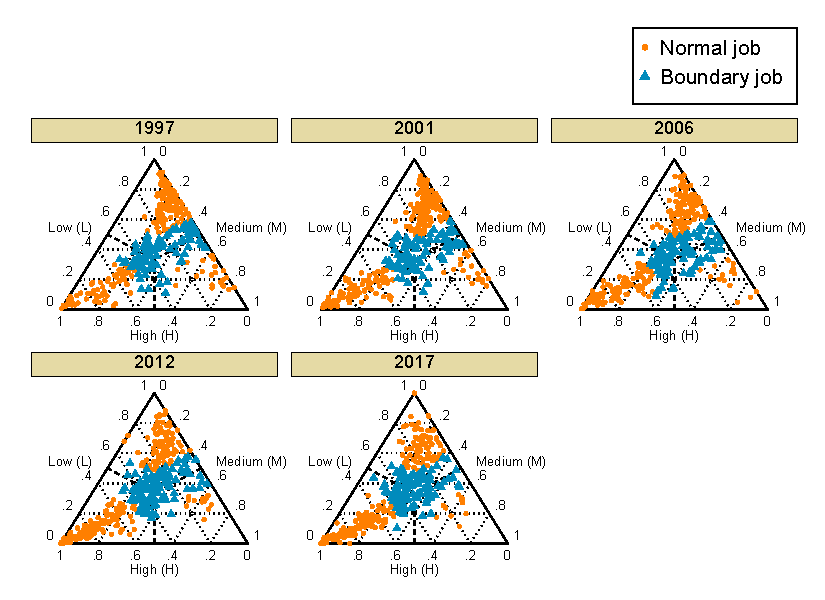
\includegraphics[width=.6\textwidth]{../output/lfsBoundary360}}
	\end{figure}
	\newpage 
	
%	\begin{center}
\begin{threeparttable}[!h]
\caption{Definition 1: share of occupations in the boundary}
\label{tab:shareBound}
\begin{tabular}{lccccc}
\toprule
\toprule
\textbf{Boundary threshold}&\multicolumn{1}{c}{\textbf{1997}}&\multicolumn{1}{c}{\textbf{2001}}&\multicolumn{1}{c}{\textbf{2006}}&\multicolumn{1}{c}{\textbf{2012}}&\multicolumn{1}{c}{\textbf{2017}} \\
\midrule
55\%        &        0.33&        0.33&        0.38&        0.39&        0.40\\
60\%        &        0.43&        0.45&        0.48&        0.49&        0.49\\
65\%        &        0.55&        0.54&        0.57&        0.60&        0.59\\
70\%        &        0.67&        0.64&        0.67&        0.69&        0.70\\
\midrule Observations&         332&         332&         332&         332&         332\\
\bottomrule
\bottomrule
\end{tabular}
\begin{tablenotes}
\item\footnotesize\textit{Note:} Source: UK Quarterly LFS. Table generated on  4 Jan 2020 at 15:35:28.
\end{tablenotes}
\end{threeparttable}
\end{center}

%	\begin{center}
\begin{threeparttable}[!h]
\caption{Definition 2: share of occupations in the boundary}
\label{tab:shareBound}
\begin{tabular}{lccccc}
\toprule
\toprule
\textbf{Boundary threshold}&\multicolumn{1}{c}{\textbf{1997}}&\multicolumn{1}{c}{\textbf{2001}}&\multicolumn{1}{c}{\textbf{2006}}&\multicolumn{1}{c}{\textbf{2012}}&\multicolumn{1}{c}{\textbf{2017}} \\
\midrule
55\%        &        0.10&        0.12&        0.10&        0.13&        0.10\\
60\%        &        0.22&        0.23&        0.23&        0.27&        0.27\\
65\%        &        0.36&        0.33&        0.35&        0.38&        0.39\\
70\%        &        0.45&        0.47&        0.48&        0.50&        0.49\\
\midrule Observations&         332&         332&         332&         332&         332\\
\bottomrule
\bottomrule
\end{tabular}
\begin{tablenotes}
\item\footnotesize\textit{Note:} Source: UK Quarterly LFS. Table generated on  4 Jan 2020 at 15:35:32.
\end{tablenotes}
\end{threeparttable}
\end{center}

%	\begin{center}
\begin{threeparttable}[!h]
\caption{Definition 3: share of occupations in the boundary}
\label{tab:shareBound}
\begin{tabular}{lccccc}
\toprule
\toprule
\textbf{Boundary threshold}&\multicolumn{1}{c}{\textbf{1997}}&\multicolumn{1}{c}{\textbf{2001}}&\multicolumn{1}{c}{\textbf{2006}}&\multicolumn{1}{c}{\textbf{2012}}&\multicolumn{1}{c}{\textbf{2017}} \\
\midrule
55\%        &        0.12&        0.14&        0.14&        0.16&        0.16\\
60\%        &        0.28&        0.27&        0.29&        0.32&        0.32\\
65\%        &        0.39&        0.42&        0.44&        0.44&        0.44\\
70\%        &        0.55&        0.54&        0.55&        0.57&        0.56\\
\midrule Observations&         332&         332&         332&         332&         332\\
\bottomrule
\bottomrule
\end{tabular}
\begin{tablenotes}
\item\footnotesize\textit{Note:} Source: UK Quarterly LFS. Table generated on 13 Jan 2020 at 13:02:19.
\end{tablenotes}
\end{threeparttable}
\end{center}

	
%	\subsection{Jobs by education-pair border}	
%	\begin{center}
\begin{threeparttable}[!h]
\caption{Definition 1: number of occupations by boundary type}
\label{tab:shareBound}
\begin{tabular}{lccccc}
\toprule
\toprule
\textbf{Boundary threshold}&\multicolumn{1}{c}{\textbf{1997}}&\multicolumn{1}{c}{\textbf{2001}}&\multicolumn{1}{c}{\textbf{2006}}&\multicolumn{1}{c}{\textbf{2012}}&\multicolumn{1}{c}{\textbf{2017}} \\
\midrule
Low-Mid     &          63&          77&          75&          76&          62\\
Mid-High    &          26&          30&          27&          31&          34\\
Low-High    &          54&          41&          58&          57&          67\\
\bottomrule
\bottomrule
\end{tabular}
\begin{tablenotes}
\item\footnotesize\textit{Note:} Source: UK Quarterly LFS. Table generated on  4 Jan 2020 at 15:35:28.
\end{tablenotes}
\end{threeparttable}
\end{center}

%	\begin{center}
\begin{threeparttable}[!h]
\caption{Definition 2: number of occupations by boundary type}
\label{tab:shareBound}
\begin{tabular}{lccccc}
\toprule
\toprule
\textbf{Boundary threshold}&\multicolumn{1}{c}{\textbf{1997}}&\multicolumn{1}{c}{\textbf{2001}}&\multicolumn{1}{c}{\textbf{2006}}&\multicolumn{1}{c}{\textbf{2012}}&\multicolumn{1}{c}{\textbf{2017}} \\
\midrule
Low-Mid     &          33&          39&          36&          42&          31\\
Mid-High    &          14&          15&          12&          19&          15\\
Low-High    &          25&          21&          30&          28&          42\\
\bottomrule
\bottomrule
\end{tabular}
\begin{tablenotes}
\item\footnotesize\textit{Note:} Source: UK Quarterly LFS. Table generated on  4 Jan 2020 at 15:35:32.
\end{tablenotes}
\end{threeparttable}
\end{center}

%	\begin{center}
\begin{threeparttable}[!h]
\caption{Definition 3: number of occupations by boundary type}
\label{tab:shareBound}
\begin{tabular}{lccccc}
\toprule
\toprule
\textbf{Boundary threshold}&\multicolumn{1}{c}{\textbf{1997}}&\multicolumn{1}{c}{\textbf{2001}}&\multicolumn{1}{c}{\textbf{2006}}&\multicolumn{1}{c}{\textbf{2012}}&\multicolumn{1}{c}{\textbf{2017}} \\
\midrule
Low-Mid     &          41&          42&          43&          51&          35\\
Mid-High    &          17&          18&          18&          21&          23\\
Low-High    &          34&          28&          35&          35&          49\\
\bottomrule
\bottomrule
\end{tabular}
\begin{tablenotes}
\item\footnotesize\textit{Note:} Source: UK Quarterly LFS. Table generated on 13 Jan 2020 at 13:02:20.
\end{tablenotes}
\end{threeparttable}
\end{center}

	
%	\subsection{Time in the border}
%	\begin{table}[h!]
	\caption{Definition 1: number of years in the border}
	\centering
	\begin{tabular}{lr}
	\toprule
Number of years & Number of jobs \\
\midrule
0&88 \\
1&49 \\
2&40 \\
3&41 \\
4&44 \\
5&70 \\
Total&332 \\
\bottomrule
\end{tabular}
\end{table}

%	\begin{table}[h!]
	\caption{Definition 2: number of years in the border}
	\centering
	\begin{tabular}{lr}
	\toprule
Number of years & Number of jobs \\
\midrule
0&156 \\
1&55 \\
2&56 \\
3&35 \\
4&20 \\
5&10 \\
Total&332 \\
\bottomrule
\end{tabular}
\end{table}

%	\begin{table}[h!]
	\caption{Definition 3: number of years in the border}
	\centering
	\begin{tabular}{lr}
	\toprule
Number of years & Number of jobs \\
\midrule
0&138 \\
1&53 \\
2&57 \\
3&35 \\
4&27 \\
5&22 \\
Total&332 \\
\bottomrule
\end{tabular}
\end{table}


	
%	\input{../output/borderExamples1.tex}
	\input{../output/borderExamples2.tex}
%	\input{../output/borderExamples3.tex}
	
%	\section{Going back to SES}
%	\bitem
%	\item I have 192 out of 332 occupations which I can track throughout the whole period.
%	\item Occupations appearing only 4 times across the period could be an issue. They account for about 25\% of employment in the \href{https://www.dropbox.com/s/bzkjsuhid0z5yaf/sesPanelEmpshare.txt?dl=0}{LFS}.
%	\bitem 
%	\item Out of these: those not appearing in 1997 are the issue. They account for about 22\% of total employment in the LFS.
%	\item Those that are missing in a year other than 1997 are probably just due to sampling. They are fairly small so I am very confident excluding them.
%	\eitem
%	\item Missing occupations after 1997 are probably the result of sampling error. They are generally small and account at most for 2\% of LFS employment.
%	\item Crux of the issues are in the change between 1997 and 2001.
%	\eitem
\end{document}

